\section{最小距离}
\label{sec:ccode-min-distance}

重复码能纠正$t$个翻转，是因为两个码字相差$2t+1$位：从一个码字出发翻转$t$位，离它仍比离另一个码字近。这个观察不依赖于“重复”本身。对任意一个二元码本，两条码字相差几位，决定了翻转之后它们还能不能被区分。

\paragraph{Hamming距离与最小距离}
长度为$n$的二元串记作行向量$\bm{x}$，它的分量是$x_1,\dots,x_n$，全体这样的串记作$\{0,1\}^{n}$。两个串取值不同的位置个数记作$\operatorname{dist}(\bm{x},\bm{y})$，称为\term{Hamming距离}（Hamming distance）。它满足非负、对称、只在$\bm{x}=\bm{y}$时为零，以及三角不等式：$\bm{x},\bm{z}$不同的每个位置上，$\bm{y}$必与其中之一不同，所以这个位置至少计入$\operatorname{dist}(\bm{x},\bm{y})$与$\operatorname{dist}(\bm{y},\bm{z})$之一。这些性质的一般讨论可参考\BookChapterRef{chap:metric-spaces}{卷四第2章“度量空间”}。串中$1$的个数记作$\operatorname{wt}(\bm{x})$，称为\term{Hamming重量}（Hamming weight），它就是$\bm{x}$到全零串的距离。

信道翻转了哪些位置，接收块与码字就在这些位置上不同，所以翻转个数正是接收块到所发码字的Hamming距离。把码本中最近的两条码字之间的距离作为码的指标。

\begin{definition}[最小距离]
\label{def:ccode-min-distance}
设二元码本$\mathcal{C}\subseteq\{0,1\}^{n}$至少含两条码字。它的\term{最小距离}（minimum distance）是
\begin{equation}
 d_{\min}=\min\bigl\{\operatorname{dist}(\bm{c},\bm{c}'):\ \bm{c},\bm{c}'\in\mathcal{C},\ \bm{c}\neq\bm{c}'\bigr\} .
 \label{eq:ccode-dmin}
\end{equation}
\end{definition}

长度为$n$的重复码$d_{\min}=n$。再看一个本章反复使用的码本，它有$4$条长度为$5$的码字：
\[
 \mathcal{C}_5=\{00000,\ 10110,\ 01011,\ 11101\} .
\]
六对码字的距离依次计算：
\[
 \begin{gathered}
 \operatorname{dist}(00000,10110)=3,\quad \operatorname{dist}(00000,01011)=3,\\
 \operatorname{dist}(00000,11101)=4,\quad \operatorname{dist}(10110,01011)=4,\\
 \operatorname{dist}(10110,11101)=3,\quad \operatorname{dist}(01011,11101)=3 .
 \end{gathered}
\]
所以$d_{\min}=3$。它与三次重复码有相同的最小距离，码率却是$\log_24/5=0.4$，高于$\tfrac13$。

\paragraph{检测与纠正}
接收端可以做两件程度不同的事。\term{检错}（error detection）只判断接收块是不是码字：若不是，就知道出了错，可以要求重发或丢弃。\term{纠错}（error correction）还要给出发送的是哪条码字。纠错用的规则是\term{最小距离译码}（minimum-distance decoding）：把接收块判为离它最近的码字，并列时按事先约定的规则任取其一。第~\ref{chap:discrete-channel-capacity}章已经说明，在$p<\tfrac12$的二元对称信道上，码字的似然$p^{k}(1-p)^{n-k}$随距离$k$增大而减小，所以最小距离译码就是最大似然解码。

\begin{theorem}[最小距离的保证]
\label{thm:ccode-detect-correct}
设码本$\mathcal{C}$的最小距离为$d_{\min}$，发送码字$\bm{c}\in\mathcal{C}$，接收块$\bm{y}$与$\bm{c}$相差$j$位。
\begin{enumerate}
 \item 若$1\leq j\leq d_{\min}-1$，则$\bm{y}\notin\mathcal{C}$，错误一定被检测到。
 \item 若
 \begin{equation}
  j\leq t,\qquad t=\Bigl\lfloor\frac{d_{\min}-1}{2}\Bigr\rfloor ,
  \label{eq:ccode-correct-radius}
 \end{equation}
 则$\bm{c}$是离$\bm{y}$最近的唯一码字，最小距离译码一定判对。
\end{enumerate}
\end{theorem}

\begin{proof}
(1) $\bm{y}$与$\bm{c}$不同，且距离$j$小于$d_{\min}$。若$\bm{y}$是码字，它就是与$\bm{c}$不同、距离小于$d_{\min}$的码字，与最小距离的定义矛盾。

(2) 由$t$的定义，$2t\leq d_{\min}-1$，即$2t<d_{\min}$。对任一码字$\bm{c}'\neq\bm{c}$，三角不等式给出
\[
 d_{\min}\leq\operatorname{dist}(\bm{c},\bm{c}')\leq\operatorname{dist}(\bm{c},\bm{y})+\operatorname{dist}(\bm{y},\bm{c}') .
\]
移项并代入$\operatorname{dist}(\bm{c},\bm{y})=j\leq t$，得到
\[
 \operatorname{dist}(\bm{y},\bm{c}')\geq d_{\min}-j\geq d_{\min}-t>t\geq j .
\]
所以每个其他码字都比$\bm{c}$离$\bm{y}$更远，最近的码字唯一，就是$\bm{c}$。
\end{proof}

对$\mathcal{C}_5$，$d_{\min}=3$，保证检测至多$2$个翻转、纠正$1$个翻转。图~\ref{fig:ccode-distance-chain}用重复码说明两个半径怎样产生。(a)中$d_{\min}=5$，两条码字之间相隔五步，各自往中间走两步的范围不相交，所以两个翻转可以纠正；任何不超过四步的走法都到不了另一端，所以四个翻转可以检测。(b)中$d_{\min}=4$，正中间的$1100$离两端都是两步，两个翻转只能被发现，不能被纠正。

\begin{BookInlineFigure}
 \centering
 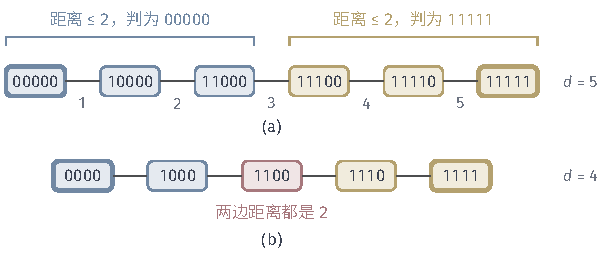
\includegraphics[width=103.2mm]{figures/07-probability/06-channel-coding/tikz/ccode-distance-chain/figure.pdf}
 \caption{沿一条每步翻转一位的路径，从一个码字走到另一个码字（粗框）。(a) 长度$5$的重复码，$d_{\min}=5$：距$00000$不超过$2$的串（蓝）判为$00000$，距$11111$不超过$2$的串（黄）判为$11111$，两部分不相交。(b) 长度$4$的重复码，$d_{\min}=4$：中间的$1100$（红）到两个码字的距离都是$2$。}
 \label{fig:ccode-distance-chain}
\end{BookInlineFigure}

\paragraph{判决球}
定理~\ref{thm:ccode-detect-correct}的第二条有一个几何读法。以码字$\bm{c}$为中心、半径为$t$的Hamming球
\[
 B(\bm{c},t)=\bigl\{\bm{y}\in\{0,1\}^{n}:\ \operatorname{dist}(\bm{y},\bm{c})\leq t\bigr\}
\]
是“翻转不超过$t$个”所能到达的全部接收块。证明中的不等式说明，当$2t<d_{\min}$时，不同码字的球互不相交：若$\bm{y}$同时在两个球内，它到两个中心的距离之和不超过$2t$，与两中心距离至少$d_{\min}$矛盾。互不相交的球给每条码字划出了一块专属的领地，落在领地里的接收块只有一种合理的解释。

图~\ref{fig:ccode-decoding-balls}是这一图景的示意。落在某个球里的接收块$y_1$被纠正到球心；落在所有球之外的$y_2$离每个码字都超过$t$，接收端知道出了错，但定理不保证它会被判对。检测的半径更大：从一个码字出发翻转不到$d_{\min}$位，到不了别的码字，所以只要接收块不是码字，就能发现错误。

\begin{BookInlineFigure}
 \centering
 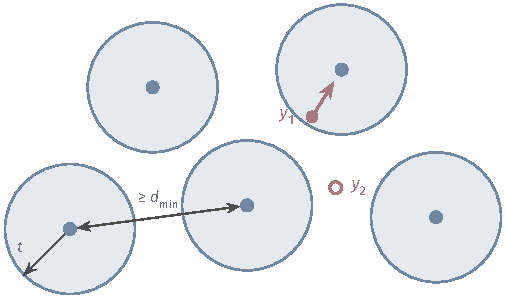
\includegraphics[width=85.7mm]{figures/07-probability/06-channel-coding/tikz/ccode-decoding-balls/figure.pdf}
 \caption{Hamming空间中判决球的示意（平面上的圆只表示“距离不超过$t$”的集合，不按真实形状绘制）。蓝点为码字，两两距离至少$d_{\min}$；浅蓝圆为半径$t=\lfloor(d_{\min}-1)/2\rfloor$的球，互不相交。红点$y_1$在球内，被纠正到球心；空心红点$y_2$不在任何球内，只能确定出了错。}
 \label{fig:ccode-decoding-balls}
\end{BookInlineFigure}

用$\mathcal{C}_5$数一数这些领地。长度为$5$的串共有$32$个，每个半径为$1$的球含中心本身和$5$个只差一位的串，共$6$个。四个球互不相交，合计$24$个串，剩下$8$个串不在任何球内。这$8$个串每个都与某两条码字相距$2$，例如$00101$到$00000$与$11101$的距离都是$2$，到另外两条码字的距离都是$3$。

\paragraph{超出半径之后}
翻转个数超过$t$时，定理不作任何承诺，但这不等于一定判错。$\mathcal{C}_5$上翻转两位后，接收块可能落进另一条码字的球里，也可能落在那$8$个“无主”的串上；后一种情形下，最小距离译码要在两条并列最近的码字中选一个，选中原码字的机会是存在的。所以超出半径后的错误概率，要按具体的信道、具体的码和具体的判决规则（包括并列时怎样选）来计算。只用保证半径计算，能得到的是错误概率的上界：在$p=0.1$时，
\[
 P_{\mathrm{e}}\leq\mathbb{P}(\text{翻转个数}\geq2)=1-0.9^5-5\times0.1\times0.9^4=0.08146 .
\]
第~\ref{sec:ccode-syndrome}小节给出一个具体的并列规则，精确算出它的错误概率。
